\documentclass[10pt,a4paper]{article}
\usepackage[T1]{fontenc}
\usepackage{tikz}
\usepackage[margin=1cm]{geometry}
\usetikzlibrary{calc,shapes.multipart,chains,arrows,positioning}
\tikzset{list/.style={very thick, rectangle split, rectangle split parts=3, draw, rectangle split horizontal, minimum size=18pt, inner sep=5pt, text=black, rectangle split part fill={blue!20, red!20, green!20}}, ->, start chain=going right, very thick}
\begin{document}
\section*{Step 1}
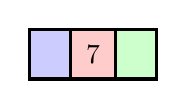
\begin{tikzpicture}
    \node[list,on chain] (N1) {\nodepart{second} 7};
\end{tikzpicture}
\section*{Step 2}
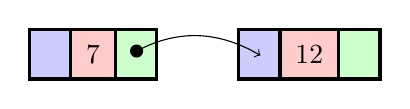
\begin{tikzpicture}
    \node[list,on chain] (N1) {\nodepart{second} 7};
    \node[list,on chain] (N2) {\nodepart{second} 12};
    \path[*->] let \p1 = (N1.three), \p2 = (N1.center) in (\x1,\y2) edge [bend left] ($(N2.one)+(0.1,0.06)$);
\end{tikzpicture}
\section*{Step 3}
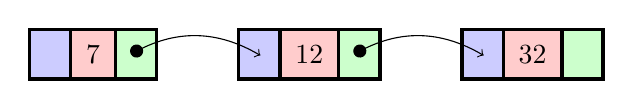
\begin{tikzpicture}
    \node[list,on chain] (N1) {\nodepart{second} 7};
    \node[list,on chain] (N2) {\nodepart{second} 12};
    \node[list,on chain] (N3) {\nodepart{second} 32};
    \path[*->] let \p1 = (N1.three), \p2 = (N1.center) in (\x1,\y2) edge [bend left] ($(N2.one)+(0.1,0.06)$);
    \path[*->] let \p1 = (N2.three), \p2 = (N2.center) in (\x1,\y2) edge [bend left] ($(N3.one)+(0.1,0.06)$);
\end{tikzpicture}
\section*{Step 4}
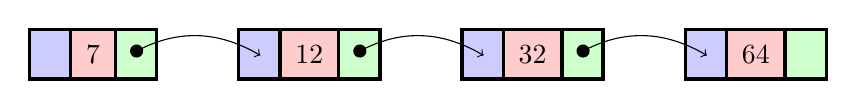
\begin{tikzpicture}
    \node[list,on chain] (N1) {\nodepart{second} 7};
    \node[list,on chain] (N2) {\nodepart{second} 12};
    \node[list,on chain] (N3) {\nodepart{second} 32};
    \node[list,on chain] (N4) {\nodepart{second} 64};
    \path[*->] let \p1 = (N1.three), \p2 = (N1.center) in (\x1,\y2) edge [bend left] ($(N2.one)+(0.1,0.06)$);
    \path[*->] let \p1 = (N2.three), \p2 = (N2.center) in (\x1,\y2) edge [bend left] ($(N3.one)+(0.1,0.06)$);
    \path[*->] let \p1 = (N3.three), \p2 = (N3.center) in (\x1,\y2) edge [bend left] ($(N4.one)+(0.1,0.06)$);
\end{tikzpicture}
\section*{Step 5}
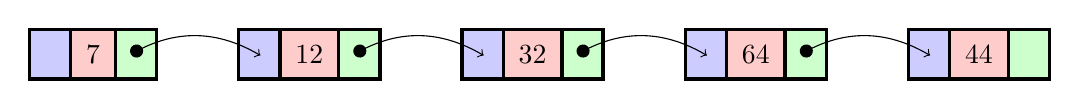
\begin{tikzpicture}
    \node[list,on chain] (N1) {\nodepart{second} 7};
    \node[list,on chain] (N2) {\nodepart{second} 12};
    \node[list,on chain] (N3) {\nodepart{second} 32};
    \node[list,on chain] (N4) {\nodepart{second} 64};
    \node[list,on chain] (N5) {\nodepart{second} 44};
    \path[*->] let \p1 = (N1.three), \p2 = (N1.center) in (\x1,\y2) edge [bend left] ($(N2.one)+(0.1,0.06)$);
    \path[*->] let \p1 = (N2.three), \p2 = (N2.center) in (\x1,\y2) edge [bend left] ($(N3.one)+(0.1,0.06)$);
    \path[*->] let \p1 = (N3.three), \p2 = (N3.center) in (\x1,\y2) edge [bend left] ($(N4.one)+(0.1,0.06)$);
    \path[*->] let \p1 = (N4.three), \p2 = (N4.center) in (\x1,\y2) edge [bend left] ($(N5.one)+(0.1,0.06)$);
\end{tikzpicture}
\section*{Step 6}
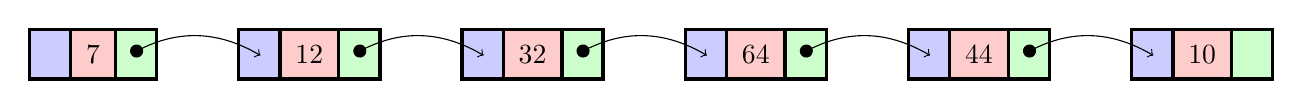
\begin{tikzpicture}
    \node[list,on chain] (N1) {\nodepart{second} 7};
    \node[list,on chain] (N2) {\nodepart{second} 12};
    \node[list,on chain] (N3) {\nodepart{second} 32};
    \node[list,on chain] (N4) {\nodepart{second} 64};
    \node[list,on chain] (N5) {\nodepart{second} 44};
    \node[list,on chain] (N6) {\nodepart{second} 10};
    \path[*->] let \p1 = (N1.three), \p2 = (N1.center) in (\x1,\y2) edge [bend left] ($(N2.one)+(0.1,0.06)$);
    \path[*->] let \p1 = (N2.three), \p2 = (N2.center) in (\x1,\y2) edge [bend left] ($(N3.one)+(0.1,0.06)$);
    \path[*->] let \p1 = (N3.three), \p2 = (N3.center) in (\x1,\y2) edge [bend left] ($(N4.one)+(0.1,0.06)$);
    \path[*->] let \p1 = (N4.three), \p2 = (N4.center) in (\x1,\y2) edge [bend left] ($(N5.one)+(0.1,0.06)$);
    \path[*->] let \p1 = (N5.three), \p2 = (N5.center) in (\x1,\y2) edge [bend left] ($(N6.one)+(0.1,0.06)$);
\end{tikzpicture}
\section*{Step 7}
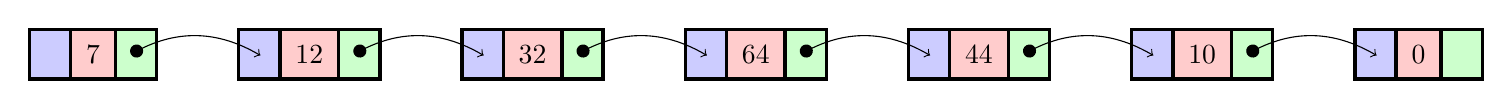
\begin{tikzpicture}
    \node[list,on chain] (N1) {\nodepart{second} 7};
    \node[list,on chain] (N2) {\nodepart{second} 12};
    \node[list,on chain] (N3) {\nodepart{second} 32};
    \node[list,on chain] (N4) {\nodepart{second} 64};
    \node[list,on chain] (N5) {\nodepart{second} 44};
    \node[list,on chain] (N6) {\nodepart{second} 10};
    \node[list,on chain] (N7) {\nodepart{second} 0};
    \path[*->] let \p1 = (N1.three), \p2 = (N1.center) in (\x1,\y2) edge [bend left] ($(N2.one)+(0.1,0.06)$);
    \path[*->] let \p1 = (N2.three), \p2 = (N2.center) in (\x1,\y2) edge [bend left] ($(N3.one)+(0.1,0.06)$);
    \path[*->] let \p1 = (N3.three), \p2 = (N3.center) in (\x1,\y2) edge [bend left] ($(N4.one)+(0.1,0.06)$);
    \path[*->] let \p1 = (N4.three), \p2 = (N4.center) in (\x1,\y2) edge [bend left] ($(N5.one)+(0.1,0.06)$);
    \path[*->] let \p1 = (N5.three), \p2 = (N5.center) in (\x1,\y2) edge [bend left] ($(N6.one)+(0.1,0.06)$);
    \path[*->] let \p1 = (N6.three), \p2 = (N6.center) in (\x1,\y2) edge [bend left] ($(N7.one)+(0.1,0.06)$);
\end{tikzpicture}
\end{document}